\chapter{User Interface Reference}\label{BasicUsage}

This section describes how to use the \ma in \textbf{interactive mode}
(graphical user interface). Most daily operations can be done that
way, actually.

However, more advanced things such as profile customization, command line
mode, etc. are described in chapter \ref{AdvancedUsage}.

\section{Launching}
Most of the commands are described with Jar files coresponding to midlets.
Unless specified otherwise, those commands also work with APK files (android
application).

\subsection*{With the mouse} On Windows, to start the analysis of
a MIDlet, just right click on its JAR or JAD file, and select ``Analyse''. It also work on an APK file. The \ma then starts in interactive mode, that is displaying its graphical user interface. An alternate way to start
the tool is \texttt{Start -> Programs -> Midlet Analyser -> Start}.

\subsection*{With the \texttt{matos} textual command}
From a Linux shell, or from a Windows DOS command prompt, the \ma can be
started using the \texttt{matos} command (the command name MATOS
stands for MIDlet Analyser Tool Suite). Ensure the \texttt{matos}
command can be found through your \texttt{PATH} environment variable:
the command is located in the installation directory on Windows, and
in the \texttt{bin} folder of the installation directory on Linux. If
no option is provided (flags such as \texttt{-h} for instance), the
\ma is started in interactive mode (GUI mode) then the analysis
process has to be launched interactively by the user. In the following
example, the tool is launched in interactive mode and prepared for analysis of the
\texttt{Pacman.jar} file: \texttt{matos Pacman.jar}. 

If at least one option is specified, the analysis starts immediately on
the file(s) provided, without opening the graphical user
interface. In that case the results are available in an HTML file, that can be
specified using the \texttt{-o} option. This is what happens on the
following example: \texttt{matos -jar Pacman.jar -o PacmanResults.html}

There are many options available with the command line mode. Please
refer to \ref{CmdLineMode} for a complete description.

\section{The Graphical User Interface}

\subsection{The Check-list Zone}
The main part of the interface is the check-list zone. It is a table
representing the current check-list, that is the sequence of analyses
that are going to be performed when you start the process. The columns
of the table represent various properties about analyses. There are
two kinds of properties, in fact: the ones that can be set by the user
to specify how the analysis must be done, and the ones that are
set by the \ma only, to feed back information about the processing of
the analysis. The first column just represents the index of the
analysis in the list, that is its step number.

There are in fact three check list zone coresponding to the different kinds of
contents analyzed by \ma : Android applications, Midlets.

\subsubsection*{Properties set by the user (MIDP specific)} The ``JAD'' and
``JAR'' columns indicate the names of the MIDlet suite files that must be analysed. By moving the mouse pointer over these columns, a tool-tip will appear showing the
full location of the file.

% The ``Profile'' column indicates what analysis profile will be used
% during the analysis; possible values are names of the profiles that
% are available in the \texttt{lib/definitions} folder of your
% installation directory.

The ``Profile'' combo box which is above the check-list table indicates what
analysis profile will be used during the analysis; possible values are names of
the profiles are available in the \texttt{lib/definitions} folder of your
installation directory.

\subsubsection*{Feedback information}
There is a narrow column titled ``M'': when a M letter appears in that
column for an analysis, it means that you have modified some
properties since the last execution of that step. This is just to warn
you that all reports generated so far for that step may no longer be
up to date. By moving the mouse pointer over a M letter, a tool-tip will appear
showing information about concerned step and in red, the difference with the last
execution.

% The ``State'' column tells you whether that step has already been executed
% (since the last time you launched the tool). When the word \texttt{Done} is
% displayed, it means that the step was executed at least once during the current
% session, and that the latest report produced is viewable from the tool; 
% \texttt{Skipped} means that an attempt to execute the step was done during the
% current session, but the process was aborted before the complete production of a
% report (failure is usually due to the fact that an input file could not be
% found, to the unavailability of a network connection, to the fact that
% the MIDlet file is not recognized as a valid one, etc).

The ``Verdict'' column tells you whether that step has already been executed and
whether the executed analysis passed or failed, with respect to the requirements
definition contained in the security profile used.
Possible values are \texttt{Passed}, \texttt{Failed} or \texttt{Skipped} if any
problem stopped analysis before the end (for instance, if the JAR file could not
be downloaded). You can modify or confirm the given verdict. If you confirm the
verdict, the cell will have a background in green. If you modify the verdict, it
is your verdict that will be in the ``Verdict'' column and the cell's background
will be in red.

Finally, the ``Comments'' column allows you adding comments associated with a
step. A cell of the ``Comments'' column will be editable after a double-click
on it.

Note : on Android, the verdict failed only means that some APIs used by the
application have not been found. Most of the time it coresponds to dead code
never trigered.

\ifthenelse{\equal{\Gallery}{true}}{

\subsection{The Editors lists Zone}
\textbf{This section is only valid for a check-list edited with a CID (Gallery
portal). } 
This part of the interface shows a table whose rows represent
editors' lists (Excel files) registered in database. The first column just represents the number 
of editor's list. For each row, columns indicate the name of the Excel file,
the editor's name, the recording's date in database, a name, an email and a
phone number of a contact if information are given in the Excel file.

}{}

%% --- RETARDE --- NYI
%% In case the ``Latest State'' information is set to \texttt{Done}, the
%% ``Latest verdict'' column tells whether the executed analysis passed
%% or failed, with respect to the requirements definition contained in
%% the security profile used. Possible values are \texttt{Passed}, \texttt{Failed} or
%% \texttt{N/A}. The latter value stands for Not Applicable and is used
%% for special profiles -- such as Agnostic -- that don't judge anything,
%% but just report neutral information about MIDlets.


\subsection{The \texttt{File}} Menu \label{FileMenu}
\begin{itemize}
\item{\textbf{New}} Clear the current check-list to create a new one.
\item{\textbf{Open}} Open an existing check-list. Check-lists are stored
in files with the \texttt{.mcl} extension. The opened check-list will
overwrite the current one.
\item{\textbf{Save}} Save the current check-list.
\item{\textbf{Save as...}} Save the current check-list to a new file.
\item{\textbf{Save selection as...}} Make a check-list of the selected
steps and save it to a new file (sub-list of the whole list).
\item{\textbf{Add File to analyse...}} Add a new analysis 
to the current check-list, by importing the target application files (midlet,
android apk). 

\ifthenelse{\equal{\Gallery}{true}}{

\item{\textbf{Register an editor's list\ldots}} Add a new editor's list by
selecting an Excel file in your hard disk. The \ma will try to import
information present in the Excel file:
\begin{itemize}
  \item Information reported in columns of the editor's list table: editor's
  name, name, email and phone number of a contact.
  \item All MIDlet suites described in the Excel file. When registering an
  editor's list, all information about MIDlet suites are only registered in
  database. To add MIDlet suites of an editor's list to the current
  check-list, select the editor's list in the \texttt{Editors lists} tab and
  click on \texttt{Add to check-list} button  above the table containing
  editor's lists.
\end{itemize} 
\item{\textbf{Register editor's lists from a directory\ldots}} Add a new row in
the editor's list table for each Excel file found in the given directory. Each
editor's list is also registered in database with its associated MIDlet suites.

}{}

\item{\textbf{Add directory...}} Add a new step for each MIDlet suite
present in a given directory. By default, the \ma behaves as follows: firstly,
the tool looks for JAD files. One step is created for each JAD file,
resolving its associated JAR with the ``Specified by JAD file'' mode,
as explained above. Secondly, every JAR file from the target directory
that has not yet been associated to a JAD during the first pass is
added alone in an extra step (\emph{orphan} JARs). An option in the
configuration's window allows to consider that a JAD file and a JAR file are
relative to the same MIDlet suite if they have the same name (like
\texttt{Pacman.jar} and \texttt{Pacman.jad}).
\item{\textbf{Add check-list...}} Add another check-list to the current
one. The selected list is appended to the end of the current one. The
tool does not check the absence of duplicate steps.
\item{\textbf{Quit}} Close the \ma.
\end{itemize}

\subsubsection{Adding a midlet}

\begin{figure}[ht]
\begin{center}
\scalebox{0.5}{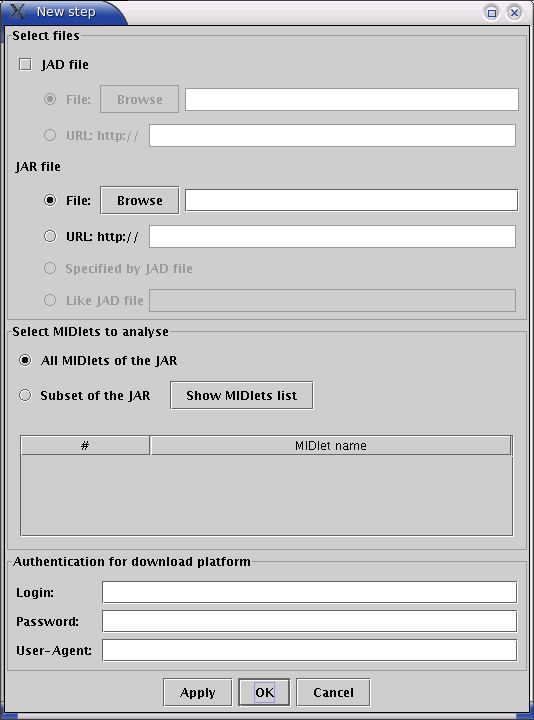
\includegraphics{figures/GUI-new-step-dialog}}
\end{center}
\caption{Specify the new step properties}
\label{figNewStep}
\end{figure} 

The properties dialog depicted on figure
\ref{figNewStep} is
raised so you can specify parameters of the new analysis. When you
click \texttt{Apply} or  \texttt{OK}, a new step will be added to the
current check-list. 

The first section of the dialog allows you to
specify the JAD and the JAR files to analyse. The JAD file is
optional, whereas the JAR is mandatory. The goal here is to inform the
\ma where to find the wanted files. To do so, you may either specify a
local path (\texttt{File}) or an HTTP address (\texttt{URL}) to the
file. If you specify a JAD file, then the location of the JAR can be
specified relative to the JAD location: you can indicate that the JAR
is to be found at the same location as the JAD's (select \texttt{Like
  JAD file} option), or at the location \emph{that is specified in the
  JAD file}, namely at the address assigned to the
\texttt{MIDlet-Jar-URL} attribute of the JAD (select \texttt{Specified by
JAD file}).

The second section lets you specify which MIDlets of the JAR file
should be analysed. Indeed, a JAR may define more than one
MIDlet object, although it often contains only one. By default, all
MIDlets of the selected JAR will be analysed (even hidden ones). To choose a
subset, select \texttt{Subset of the JAR} and press \texttt{Show MIDlets
 list}. The tool will look for the JAR file, look into it and tell you the list
 of \emph{visible} MIDlets that it contains.  
 From that point, only the MIDlets that you select from that list will be taken into account.

Some downloading platforms require an authentification to access it. The third
section allows you to specify a login, a password and a user-agent to use when
downloading JAD and JAR files. 


\subsubsection{Adding an APK}
The dialog (figure \ref{figStepAndroid}) is much simpler as there is only one
file. It is either a local file or a URL. If it is a URL, it is possible to give some credentials to perform the
download. 

\begin{figure}[ht]
\begin{center}
\scalebox{0.5}{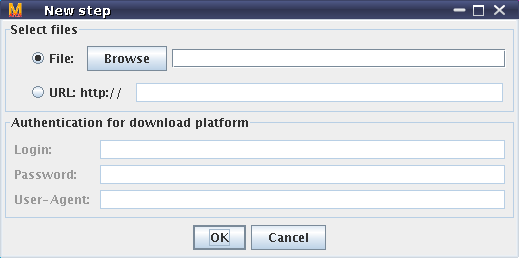
\includegraphics{figures/GUI-new-step-android}}
\end{center}
\caption{Specify the new step properties for an APK}
\label{figStepAndroid}
\end{figure} 
\subsection{The \texttt{Edit} Menu} \label{EditMenu}
\begin{itemize}
\item{\textbf{Select all}} Select all steps of the check-list.
\item{\textbf{Unselect all}} Unselect all steps of the check-list.
\item{\textbf{Copy}} Register in memory the selected steps.
\item{\textbf{Paste under}} Paste all steps previously registered with the
\texttt{Copy} option under the last selected row. 
\item{\textbf{Remove}} Remove the selected steps from the check-list.
\ifthenelse{\equal{\Gallery}{true}}{
\item{\textbf{Remove associated steps}} Remove all steps from the check-list
table which are associated with selected editor's list(s) in the editor's list
table. }{}
\item{\textbf{Properties...}} Edit the properties of the selected
step. The dialog that opens is very similar to the one used at step-creation
time (see section \ref{FileMenu}, figure \ref{figNewStep}). When you
press \texttt{Apply} or \texttt{OK}, your changes are applied to the
selected step.
\item{\textbf{Configuration...}} Edit the global configuration options of the
\ma. This window contains four tabs.
\begin{itemize}
  \item The ``Main'' tab (see figure \ref{MainTabOfConfigDialog})
	\begin{itemize}
  	 	\item \textbf{Default profile}: The default profile selected in the combo
  	box of the check-list zone at the opening of the \ma.
  		\item \textbf{Download of files} Select a proxy if it is necessary.
  		\item \textbf{Custom} The Cascading Style-Sheet (CSS) file to use for
  		pretty-presentation of the HTML reports. The default one is provided to you
  		with the \ma.
    \end{itemize}
    \begin{figure}[ht]
		\begin{center}
		\scalebox{0.5}{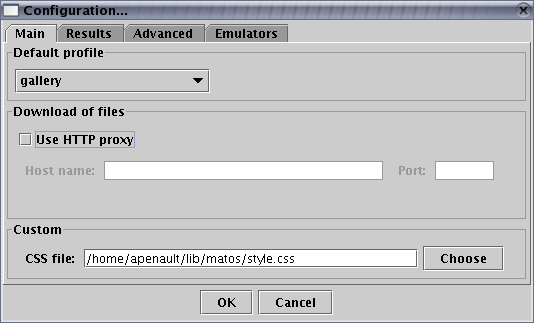
\includegraphics{figures/MainTab}}
		\end{center}
		\caption{The ``Main'' tab of the configuration's window}
		\label{MainTabOfConfigDialog}
	\end{figure}
  \item The ``Results'' tab (see figure \ref{ResultsTabOfConfigDialog})
      \ifthenelse{\equal{\Gallery}{true}}{
      	%\item \textbf{Storage}: 
      	
      
      	The first option ``Use archiving database to store analysis results''
      	allows to register all analysis results in the database. If this option
      	is selected and a connection to a database is available, you can ask to
      	the \ma to retrieve previous results from database. In that case, when a
      	step is added in the check-list, the \ma looks for previous results for
      	this JAR file in the database. If it finds a result, it displays its
      	verdict. If parameters of current step is a little different to the
      	registered result, it puts a ``M'' in the fourth column of the check-list
      	and indicates differences in associated tool tip in red. Moreover, you
      	can configure database parameters i.e. its URL (like 
      	\emph{jdbc:mysql://localhost/matos}), a user login and a user password to
      	access to the database by clicking on ``Configure database" button.
      	
      	The second option (``Use a directory to store analysis results''),
      	selected by default, allows you to select a directory to store analysis
      	results. If this option is selected, all generated reports are registered
      	in the specified directory. For more information on working of this
      	directory, please refer to \ref{HTMLReportGeneration}. 
      	
      	If you choose the ``Don't store analysis results'' option, results are
        registered in a temporary directory during the execution of the \ma,
        this directory will be deleted at the closing of the \ma.  
        
        If the first option is selected and the database connection is not
        available, the behaviour of the \ma is the same that if the third option
        is selected i.e. analysis results are stored in a temporary directory
        that is deleted at the closing of the \ma.
%         \item \textbf{Retrieving}: If a connection to a database is available, you
%         can ask to the \ma to retrieve previous results from database. If the
%         option is selected, when a step is added in the check-list, the \ma
%         looks for previous results for this JAR file in the database. If it
%         finds a
%         result, it displays its verdict. If parameters of current step is a 
%         little different to the registered result, it puts a ``M'' in the fourth
%         column of the check-list and indicates differences in associated tool
%         tip in red.
%         \item \textbf{Configure database\ldots}: This button allows you
%         configuring database parameters i.e. its URL (like
%         \emph{jdbc:mysql://localhost/matos}), a user login and a user password
%         to access to the database.
        \begin{figure}[ht]
			\begin{center}
			\scalebox{0.5}{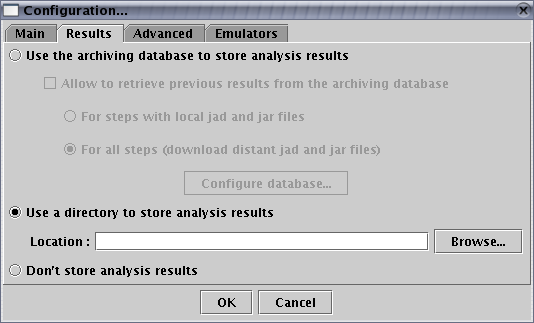
\includegraphics{figures/ResultsTabGallery}}
			\end{center}
			\caption{The ``Results'' tab of the configuration's window}
			\label{ResultsTabOfConfigDialog}
	   	\end{figure}
      }{
       By default, HTML reports are stored in the directory specified during the
       installation and all generated reports are registered in it. If you 
       choose the ``Don't store analysis results'' option, results are 
       registered in a temporary directory during the execution of the \ma, this
       directory will be deleted at the closing of the \ma. Please refer to
       \ref{HTMLReportGeneration} for information on HTML reports. \begin{figure}[ht]
			\begin{center}
			\scalebox{0.5}{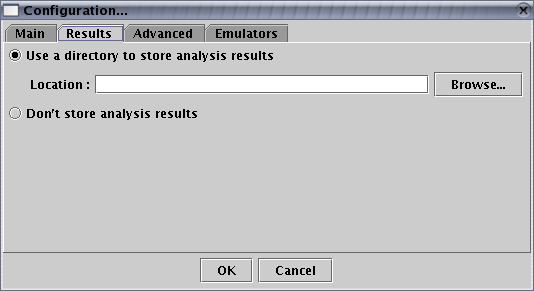
\includegraphics{figures/ResultsTab}}
			\end{center}
			\caption{The ``Results'' tab of the configuration's window}
			\label{ResultsTabOfConfigDialog}
	   	\end{figure}
	  }
  \item The ``Advanced'' tab (see figure \ref{AdvancedTabOfConfigDialog})
  	\begin{itemize}
       \item \textbf{Add directories}: If the \texttt{Yes} option is selected
       in the ``Advanced'' tab, the \ma will consider during loading a directory
       that a JAR and a JAD file which have the same name (like Pacman.jad and
       Pacman.jar) are relative to the same MIDlet suite. By default, the
       \texttt{No} option is selected.
       \begin{figure}[ht]
			\begin{center}
			\scalebox{0.5}{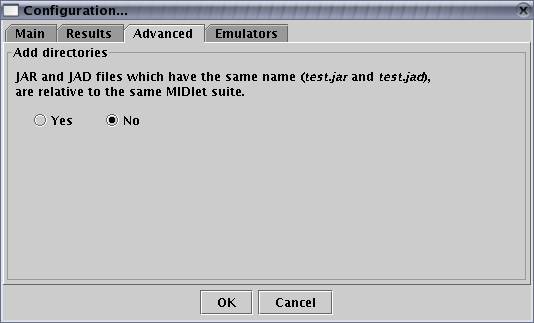
\includegraphics{figures/AdvancedTab}}
			\end{center}
			\caption{The ``Advanced'' tab of the configuration's window}
			\label{AdvancedTabOfConfigDialog}
	   	\end{figure}
      \end{itemize}
  \item Finally, the ``Emulators''tab (see figure \ref{EmulatorTabOfConfigDialog})
		
		In this tab, you can manage emulators that allow to run MIDlets of the
		check-list. The ``Add emulator'' button displays a dialog to make a link to a
		new emulator by giving a name and its command line to run it. The
		command line must contains ``\%JAD\%'' string to indicate where the path to
		the JAD must be given in it.
		The ``Remove emulator'' button allows to remove the emulator selected in the
		combo box.		
		The ``Edit emulator's properties'' button allows to modify properties of
		selected emulator i.e. its name and/or its command line.		
		The emulator selected in the combo box is the emulator run by default when you
		launch the emulator by a right click on a MIDlet suite.
		
		\begin{figure}[ht]
			\begin{center}
			\scalebox{0.5}{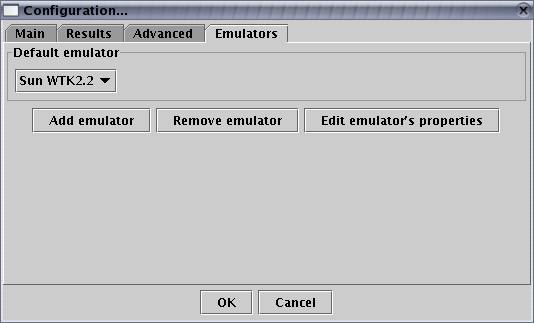
\includegraphics{figures/EmulatorTab}}
			\end{center}
			\caption{The ``Emulators'' tab of the configuration's window}
			\label{EmulatorTabOfConfigDialog}
	   	\end{figure}
\end{itemize}
\end{itemize}

\ifthenelse{\equal{\Gallery}{true}}{
\subsection{The \texttt{View} Menu}
The editor's list gives more information about MIDlet suite than information
given by columns of the check-list table. You can see all retrieved information
from Excel files by selecting \texttt{Complete information} in the \texttt{View}
menu. By default, the showed view is \texttt{Basic information} which contains
uniquely previously described columns. The columns added by selecting
\texttt{Complete information} are:

\begin{itemize}
\item{\textbf{EL\#}} Number of associated editor's list.
\item{\textbf{Name}} Name given by the editor to the MIDlet suite.
\item{\textbf{SMS}} True if the MIDlet suite makes SMS connection(s).
\item{\textbf{Authorized URLs}} By default, HTTP connections are forbidden. To
authorize HTTP connections to some URLs, the editor can declare these URLs in
the editor's list.
\item{\textbf{Service}} Name of editor's service.
\item{\textbf{Version}} Version of the given MIDlet suite.
\item{\textbf{Terminal}} Compatible devices with this MIDlet suite.
\end{itemize}
}{}

\subsection{The \texttt{Tools} Menu}
\begin{itemize}
\item{\textbf{View latest report}}: Displays the latest generated report for
the selected step.
\item{\textbf{View JAD}}: Displays the contents of the JAD file associated
to the selected step.
\item{\textbf{View JAR manifest}}: Displays the contents of the JAR manifest 
file associated to the selected step.
\item{\textbf{Analyse selection}}: Starts the analysis process for
the selected step(s) only. 
\item{\textbf{Analyse all}}: Starts the execution of the entire
check-list. All steps are processed.
\item{\textbf{Confirm the verdict}}: You can confirm the verdict given by the
\ma. In that case, the verdict's cell appears with a green background.
\item{\textbf{Modify the verdict}}: You can also modify the verdict given by the
\ma. The verdict in the ``Verdict'' column will be the verdict given by you and
the cell's background will be in red.
\item{\textbf{View statistics}}: Displays a graphic which represents verdicts in
the current check-list.
\item{\textbf{View log file}}: You can show trace generated by the \ma showing
this file.
\ifthenelse{\equal{\Gallery}{true}}{
\item{\textbf{Management tools}}: This menu allows to access to the database
management tool. It enables you showing and removing information registered in
database. To have more details, see section \ref{databaseManagementTool}.
}{}    
\item{\textbf{Launch selected MIDlet suite}}: Displays a submenu which contains
the name of available emulators. You could add a new emulator by clicking on
``Add emulator\ldots'' button and giving a name and its command line to run it.
\end{itemize}

\subsection{The \texttt{Packages} Menu}
This menu allows to select what set of Java distributions (JSRs) must be taken
into account during analysis. In general, keep \texttt{all} selected.

\subsection{The \texttt{Help} Menu}
\begin{itemize}
%\item{\textbf{User's manual}}: Opens the online help.
\item{\textbf{About}}: General information about the \ma tool.
\end{itemize}

\ifthenelse{\equal{\Gallery}{true}}{

\subsection{ The Database Management Tool} \label{databaseManagementTool}

The Database Management Tool is composed in three parts and a menu bar. It
allows to view results stored in database by selecting criteria and gives the
possibility to remove results from the database.

\subsubsection{Selection criteria}

The ``Criteria'' panel (see figure \ref{criteriaPanel}) allows to give selection
criteria to retrieve steps from database and to display them in the ``Results''
panel.

The selection criteria are:
\begin{itemize}
  \item{\textbf{Profile}} the analysis profile.
  \item{\textbf{Version}} the version of selected profile.
  \item{\textbf{Verdict}} the verdict given by the \ma.
  \item{\textbf{User verdict}} the user verdict i.e. if the verdict given by the
  \ma is confirmed, modified by you or you don't put your own verdict for these
  steps.
  \item{\textbf{Midlet Analyser release}} release of the \ma.
  \item{\textbf{JAR name}} you have three possibilities to give name of JAR file
  you want to retrieve from database. Either you give a part of JAR name or
  the beginning or the end of JAR name.
  \item{\textbf{Date}} you can also retrieve steps by creation date of results.
\end{itemize}

\begin{figure}[ht]
	\begin{center}
	\scalebox{0.5}{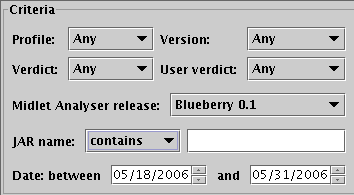
\includegraphics{figures/CriteriaPanel}}
	\end{center}
	\caption{``Criteria'' panel of the Database Management Tool}
	\label{criteriaPanel}
\end{figure}

\subsubsection{Steps' presentation}

Steps retrieved from database are displayed in the ``Results'' panel. To update
the list of steps after a modification of criteria, click on the ``Refresh''
green button above this panel. The table in this panel is similar to the table
in the check-list zone but another column indicates the creation date of
analysis reports (see figure \ref{resultsPanel}).

\begin{figure}[ht]
	\begin{center}
	\scalebox{0.5}{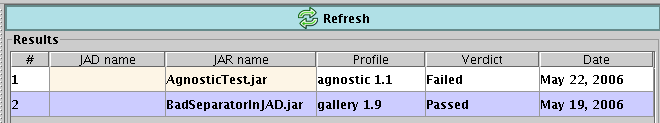
\includegraphics{figures/resultsPanel}}
	\end{center}
	\caption{``Results'' panel of the Database Management Tool}
	\label{resultsPanel}
\end{figure}

\subsubsection{Step's properties}

A third panel allows to display properties by selecting a step in ``Results''
panel (see figure \ref{stepProperties}).

\begin{figure}[ht]
	\begin{center}
	\scalebox{0.5}{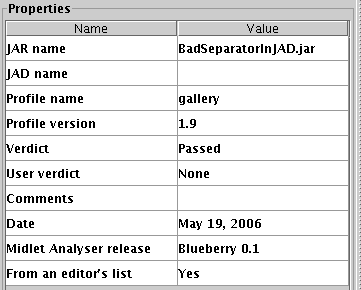
\includegraphics{figures/stepPropertiesPanel}}
	\end{center}
	\caption{``Properties'' panel of the Database Management Tool}
	\label{stepProperties}
\end{figure}

\subsubsection{Menus}

\begin{itemize}
  \item{\textbf{File -> Quit}} Close the Database Management Tool.
  \item{\textbf{Edit}}
	\begin{itemize}
      \item{\textbf{Select all}} Select all steps of the results' table.
      \item{\textbf{Unselect all}} Unselect all steps of the results' table.
      \item{\textbf{Remove selection}} Remove selected step(s) from database.
      \item{\textbf{Remove by date\ldots}} Display a window which enables to
      remove either all steps whose creation date is between two dates or before
      a specified date or older than \emph{n} days.
      \item{\textbf{Database properties\ldots}} Display a window which enables to
      configure the database URL, the database user login and the database user password.
    \end{itemize}
  \item{\textbf{Tools -> View report}} Enable to view the analysis report of the
  selected step.
\end{itemize}

}{}

\section{Analysis Profiles}\label{AnaProfs}

Most of the analysis done by the \ma is performed according to an
analysis profile. An analysis profile is a text file where directives
for the tool are specified, where you can define what the analysis must
focus on, and also how the results of the analysis should be
presented. Multiple profiles can be defined for different purposes,
but the \ma is always bound to a single profile at a time. 

An analysis profile can be seen as the implementation of a
set of analysis rules. The profile describes, in short terms, what
Java methods and arguments must be studied (it declares sort of
``probes'' on these objects), and according to the results observed,
what text messages must be produced in the report. However, in
contrast to a probe which usually provides a sample of the possible
objects states (a thermometer, for instance, indicates the current
temperature, but not tomorrow's temperature), the \ma's probes give
you a pattern covering all possible states, taking into
account all possible executions of the application. The pattern tries
to stick as much as possible to the real set of possible values, but
in general this exact set of values can not be computed; that's why
the analysis returns an upper approximation of the set, to make sure
at least that all possible values are captured.

Modifying a profile should be done very carefully, since it widely
determines the analysis engine's behaviour. If you deal with the
analysis of particularly critical features, make sure your
specification of the associated rules is correct and won't lead to
confusion between what you had in mind and what the tool
understands. On the other hand, this open approach is very flexible
and allows to highly customize the targets, preciseness and
presentation of your reports. We recommend that you contact us for
assistance if you wish to do changes to your profile, or define your
own profile from scratch. Section \ref{ProfFormalization} presents how
to formalize a profile.


\subsection{The MIDP Agnostic profile}

The \ma comes with a predefined profile called Agnostic. Its purpose
is to report the use of a set of potentially critical features, mainly
related to inputs/outputs (I/O) : network connections, system properties queries, Record Management
System (RMS), multimedia players, etc. The main characteristic of the Agnostic
profile is that results are not judged: there's no notion of pass or
fail, but just reporting.

The observed methods are the following, with the observed argument(s)
shown in bold-face when there are more than one:

\begin{itemize}
\item \texttt{javax.microedition.io.Connector.open(java.lang.String)}
\item \texttt{javax.microedition.io.Connector.open(\textbf{java.lang.String},int)}
\item \texttt{javax.microedition.io.Connector.open(\textbf{java.lang.String,int},boolean)}
\item \texttt{javax.microedition.io.Connector.openDataInputStream(java.lang.String)}
\item \texttt{javax.microedition.io.Connector.openDataOutputStream(java.lang.String)}
\item \texttt{javax.microedition.io.Connector.openInputStream(java.lang.String)}
\item \texttt{javax.microedition.io.Connector.openOutputStream(java.lang.String)}
\item \texttt{javax.wireless.messaging.MessageConnection.newMessage\\ \mbox{} \hspace{1cm} (java.lang.String,\textbf{java.lang.String})}
\item \texttt{javax.wireless.messaging.Message.setAddress(java.lang.String)}
\item \texttt{com.siemens.mp.gsm.SMS.send(\textbf{java.lang.String},java.lang.String)}
\item \texttt{com.siemens.mp.gsm.SMS.send(\textbf{java.lang.String},byte[])}
\item \texttt{com.siemens.mp.io.Connection(java.lang.String)}
\item \texttt{javax.microedition.media.Manager.createPlayer(java.lang.String)}
\item \texttt{javax.microedition.media.Manager.createPlayer\\ \mbox{} \hspace{1cm} (javax.microedition.media.protocol.DataSource)}
\item \texttt{javax.microedition.media.protocol.DataSource(java.lang.String)}
\item \texttt{javax.microedition.rms.RecordStore.openRecordStore\\ \mbox{} \hspace{1cm} (java.lang.String,boolean,\textbf{int},boolean)}
\item \texttt{javax.microedition.rms.RecordStore.setMode(\textbf{int},boolean)}
\item \texttt{java.lang.System.getProperty(java.lang.String)}
\item \texttt{java.lang.Class.forName(java.lang.String)}
\item \texttt{javax.microedition.midlet.MIDlet.platformRequest(java.lang.String)}
\end{itemize}


\section{Analysis Reports}

When you select a step in the check-list then ask \texttt{View latest
report}, a tab in your default browser will open to display the latest results
of that analysis. Note that the presentation style can be customized by changing the CSS file
(cf. \ref{EditMenu}). In this section we explain the structure of a
report, and how reports are stored on your disk, so you can open them
outside of the \ma application.

\subsection{Structure of a Report}

A MIDP report mainly contains three sections.

\begin{itemize}
\item\textbf{Header}: General information on the analysis.
\item\textbf{Descriptors conformity}: Remarks on JAD file and JAR manifest
  validity, and if both are given, on their consistency. 
\item\textbf{Per-MIDlet results}: For each MIDlet analysed, this section
  presents all remarks coming out of the Features Usage analysis
  phase. Messages displayed at that level are
  defined in the analysis profile used. 
\end{itemize}

An Android report mainly contains two sections.
\begin{itemize}
  \item \textbf{Header}: General information extracted from the manifest
  \item \textbf{A global analysis} of the APK. 
\end{itemize}
It is possible to get a per component analysis of an APK but it is not clear
that this distinction is worth the effort (the analysis time is almost
multiplied by the number of components).

% \subsection{The \texttt{Report} window} \label{ReportWindowSection}
% 
% This window gives access to a \texttt{File menu} which contains three options: 
% \begin{itemize}
%   \item \textbf{Export report in HTML\ldots} Display a dialog which allows to select
%   an HTML file to save the report.
%   \item \textbf{Export report in PDF\ldots} Display a dialog which allows to select
%   a PDF file to save the report.
%   \item \textbf{Close} Close this window. You can also close it by
%   clicking on the \texttt{Close} button at the bottom of this window.
%   \begin{figure}[ht]
% 	\begin{center}
% 	\scalebox{0.5}{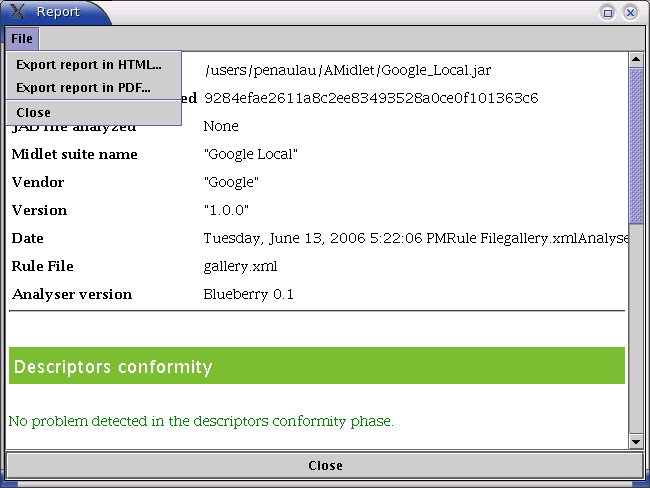
\includegraphics{figures/ReportWindow}}
% 	\end{center}
% 	\caption{The ``Report'' window}
% 	\label{ReportWindow}
%   \end{figure}
% \end{itemize}

\subsection{Using Reports Outside of the Tool} \label{HTMLReportGeneration}

If you chose to store analysis results in a directory in the configuration's
window (see section \ref{EditMenu}), the \ma will create
a sub-folder called \texttt{AnalysesResults} into the specified directory at the
first analysis. In the \texttt{AnalysesResults} folder the tool then generates a
new subfolder \texttt{Results\emph{<i>}} for each new execution of the analysis
process, ie. for each new execution of a check-list.
 
For each execution, there are: 
\begin{itemize}
\item one HTML report per step executed, and
\item one summary file (\texttt{index.html}) pointing to all the HTML reports
\end{itemize}

% As the execution of the
% check-list goes along, the \ma creates a sub-folder called
% \texttt{AnalysesResults} into \textbf{output directory} specified in the
% configuration of the tool. Refer to section \ref{EditMenu} to learn how to
% customize the output directory. 
% In the \texttt{AnalysesResults} folder the tool then generates a new
% subfolder \texttt{Results\emph{<i>}} for each new execution of the
% analysis process, ie. for each new execution of a check-list. The
% \emph{i} counter contains all result files for the execution number \emph{i}, namely:
% \begin{itemize}
% \item one HTML report per step executed, and
% \item one summary file (\texttt{index.html}) pointing to all the HTML reports
% \end{itemize}

If you open \texttt{index.html} in your HTML
browser, you'll find something very similar to the check-list zone
available in the GUI. You can then print reports from there. It is the
responsibility of the user to clean the execution folders
that are no longer needed.

% If you chose the ``Don't store analysis results'' option in the configuration's
% window, you can still save results explicitely choosing \texttt{File -> Export
% report in HTML\ldots} or \texttt{File -> Export report in PDF\ldots} menu in
% the \texttt{Report} window (see section \ref{ReportWindowSection}).

 %%% Local Variables: 
%%% mode: latex
%%% TeX-master: "Users-manual"
%%% End: 
